%% GENERATED FILE -- do not edit.
%% Written by scripts/manuscript/to_latex.py from manuscript/MANUSCRIPT_BMB_v5.md.
%% The markdown is the source; every number in it is recomputed by a script in
%% scripts/ and asserted by tests/.
%%
%% CLASS: Springer Nature sn-jnl, vendored at manuscript/springer/sn-jnl.cls
%% (LPPL). The option is sn-mathphys-ay -- AUTHOR-YEAR, which is what Bulletin of
%% Mathematical Biology uses and how the reference list below is written. The
%% Springer template ships with sn-mathphys-num uncommented; selecting it would
%% silently reformat the reference list into numbered style and break every
%% in-text citation, which are author-year throughout.
\documentclass[pdflatex,sn-mathphys-ay]{sn-jnl}

%% the class loads fontenc, geometry, hyperref, natbib, amsthm and others itself
\usepackage{amsmath,amssymb}
\usepackage{graphicx}
\usepackage[export]{adjustbox}
\usepackage{booktabs}
\usepackage{longtable}
\usepackage{array}
\usepackage{textcomp}

\usepackage{newunicodechar}
%% pandoc marks an uncaptioned longtable with \LTcaptype{none}; the caption
%% package then tries to step a counter of that name. Declaring it makes the
%% marker the no-op pandoc intends rather than a fatal error.
\newcounter{none}

\setlength{\emergencystretch}{3em}
\providecommand{\tightlist}{%
  \setlength{\itemsep}{0pt}\setlength{\parskip}{0pt}}

%% unicode that survives into prose, mapped from this document's own inventory
\newunicodechar{²}{$^{2}$}
\newunicodechar{¹}{$^{1}$}
\newunicodechar{×}{$\times$}
\newunicodechar{⁰}{$^{0}$}
\newunicodechar{⁷}{$^{7}$}
\newunicodechar{⁹}{$^{9}$}
\newunicodechar{⁻}{$^{-}$}
\newunicodechar{−}{$-$}
\renewcommand{\thefigure}{S\arabic{figure}}
\renewcommand{\topfraction}{0.92}
\renewcommand{\textfraction}{0.06}
\renewcommand{\floatpagefraction}{0.85}

\title[Fold condition for quality-control models]{An Exact Fold Condition for Mass-Balanced Models
       of Protein Quality Control}
\author*[1]{\fnm{Kiran} \sur{Boggavarapu}}\email{kiran@mcneese.edu}
\equalcont{ORCID 0000-0003-0751-6459}
\affil*[1]{\orgdiv{Department of Chemistry and Physics}, \orgname{McNeese State University}, \orgaddress{\city{Lake Charles}, \state{LA}, \postcode{70609}, \country{USA}}}


\abstract{Supplementary material accompanying the paper above. Every number in the caption is recomputed by the script named in it and asserted by the accompanying test suite.}

\begin{document}
\maketitle

\begin{figure}[htbp]
\centering
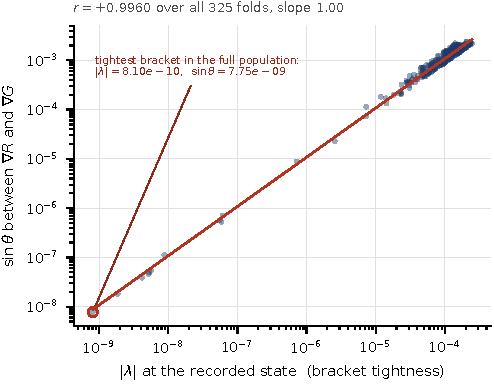
\includegraphics[max width=\linewidth]{../figures/figS1.pdf}
\caption{Parallelism residual against leading eigenvalue, over all 325 load-grid folds with no subsample. The correlation is +0.9960 in log-log with slope 1.000, so $\sin (angle)$ is proportional to bracket looseness rather than merely increasing with it; the tightest-bracketed state has $|\lambda |$ = 8.10×10⁻¹⁰ and $\sin (angle)$ = 7.75×10⁻⁹. The figure also carries the normalisation contrast: normalising by $\max (|\det J|, |\operatorname{cross}|)$ is $0/0$ at an exact fold, and that residual degrades as the bracket tightens (median 3.133×10⁻⁷ on the tighter half against 1.455×10⁻⁷ on the looser, 2.15× worse where it matters most, log-log correlation −0.835, maximum 1.54×10⁻²), whereas the gradient normalisation used throughout correlates at +0.041 with a maximum of 1.29×10⁻⁹.}
\label{fig:figS1}
\end{figure}

\begin{figure}[htbp]
\centering
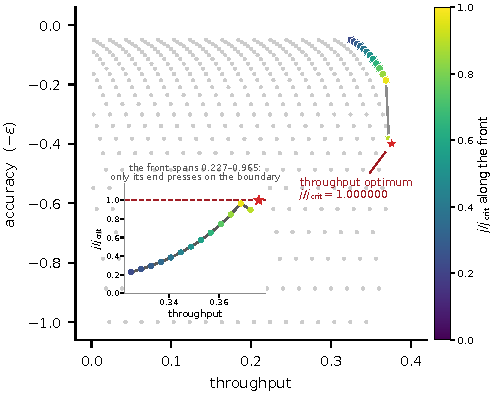
\includegraphics[max width=\linewidth]{../figures/figS2.pdf}
\caption{Strategy space cut by the fold condition: 469 feasible strategies, 13 non-dominated, with $j/j_{crit}$ running 0.2271 to 0.9652 along the front (median 0.5010). The exact throughput optimum sits at $j/j_{crit}$ = 1.000000 exactly, on the feasibility boundary; the best grid strategy reaches 0.897488, the gap being discretisation of the grid rather than an interior optimum. Supplementary Section S1 develops a strategy-space consequence of the fold condition: cutting a two-coordinate trade-off surface by the constraint $j(\alpha ,R) < j_{crit}(R)$ places the throughput optimum exactly on the feasibility boundary, while along the non-dominated front $j/j_{crit}$ runs 0.227 to 0.965.}
\label{fig:figS2}
\end{figure}

\begin{center}\rule{0.5\linewidth}{0.5pt}\end{center}

\end{document}
